\headline{{\textbf{\Large\sffamily The Top Chop:}}\\
          {\textbf{\large\sffamily The Tree of the Month Competition}}}
\label{2025-12-totm}
\noindent
December's meeting brought a festive sparkle to our benches as members embraced the holiday spirit for our final gathering of the year.
The theme, \textit{``Festive fun \& Party time!''}, inspired a delightful range of creative displays, proving that bonsai can indeed join in the seasonal celebrations.
From miniature lights to winter scenes, the trees were dressed to impress, creating a joyful atmosphere of camaraderie and lighthearted competition.

\medskip
\noindent
For those joining us, here is a brief summary of how our competition works.
All attending members are encouraged to vote on every tree presented, excluding their own, to ensure a consistent and fair spread of votes.
Each member awards between 1 (lowest) and 3 (highest) points across four categories: \textbf{trunk and branch structure}, \textbf{foliage quality}, \textbf{pot suitability}, and \textbf{overall presentation and interpretation of the theme}.

\noindent
Total scores are calculated by summing these points to determine the monthly ranking for both categories.
Usually, these positions grant points toward our yearly rankings; however, as the December theme is purely for fun, scores are not being recorded for the annual league table this month.
For the full ruleset, please refer to the \textbf{November 2025 newsletter}.

\medskip
\topic{General Tree of the Month}
\noindent
The General category featured seasoned trees with a holiday twist, showcasing how well our members can balance horticultural skill with festive creativity.

\begin{enumerate}
    \item \textbf{Terry Wilson}'s Juniper (\textit{`Juniperus'}, 5+ years old) --- A tall, formal upright specimen adorned with multi\--colored fairy lights and various festive baubles, standing proudly in a mica pot on a traditional dark wood stand.
    \item \textbf{Tina Todd}'s Cotoneaster (\textit{`Cotoneaster microphyllus'}) --- A creative winter scene featuring vibrant red berries contrasted against white ``snow'' batting, complete with small elf figurines and a large glittery ``Merry Christmas'' sign next to its Nick Payne's pot.
    \item \textbf{Steve Palmer}'s White Spruce (\textit{`Picea Glauca'}, 10 years old) --- A rugged tree styled with silver tinsel and red snowflakes, featuring a small wrapped gift nestled into the moss at its base on a natural slate slab.
\end{enumerate}

\noindent
Congratulations to \textbf{Terry Wilson} for claiming the top spot in this month's festive display!

\medskip
\topic{Novice Tree of the Month}
\noindent
Our Novice members rose to the occasion with great enthusiasm, presenting trees that captured the essence of the season perfectly.

\begin{enumerate}
    \item \textbf{Edward Mason}'s Himalayan Juniper (\textit{`Juniperus Squamata'}, 4 years old) --- A dramatic semi\--cascade tree styled with elegant red and gold baubles, presented in a textured turquoise pot by Nick Payne on a decorative red snowflake mat.
    \item \textbf{Martin Redfern}'s European Larch (\textit{`Larix Decidua'}) --- A slender, curving trunk decorated with delicate hanging ornaments and wrapped in warm white lights, finished with a bright red bow around the pot and a miniature Santa figure.
\end{enumerate}

\noindent
Well done to our Novice winner, \textbf{Edward Mason}, for his festive Juniper!

\vspace*{-0.5em}
\begin{center}
$\cdots$
\end{center}
\vspace*{-0.5em}

\noindent
This festive round was a wonderful way to close out our year, reminding us of the joy and fun at the heart of our hobby.
As we look toward the New Year, our January theme takes us back to basics: \textit{``Naked tree, Elm.''}.
This will be a fantastic opportunity to appreciate the intricate ramification and winter silhouettes of our deciduous trees.

See you all in January!
\closearticle
\headline{{\textbf{\Large\sffamily Wood You Believe It?}}\\
          {\textbf{\large\sffamily Cultivating Your Bonsai IQ}}}

\begin{itemize}
    \item \textbf{The Oldest Bonsai:} The Ficus retusa Linn at the Crespi Bonsai Museum in Italy is estimated to be over \textbf{1,000 years old}.

    \item \textbf{Etymology:} The word ``Bonsai'' (\begin{CJK*}{UTF8}{bsmi}盆栽\end{CJK*}) literally translates to \textbf{``Tray Planting.''}
    \textit{Bon} is the tray/pot, and \textit{Sai} is the planting/planting material.

    \item \textbf{Deadwood:} The white, stripped wood on a bonsai is called \textbf{Jin} (a dead branch) or \textbf{Shari} (deadwood on the trunk).
    In nature, this happens via lightning or harsh mountain winds.

    \item \textbf{The Bow:} A bonsai's \textbf{``front''} is (also) determined by the trunk's lean.
    The tree should ``bow'' slightly toward the viewer as a sign of welcome.
\end{itemize}

\closearticle

\vfill
\begin{center}
	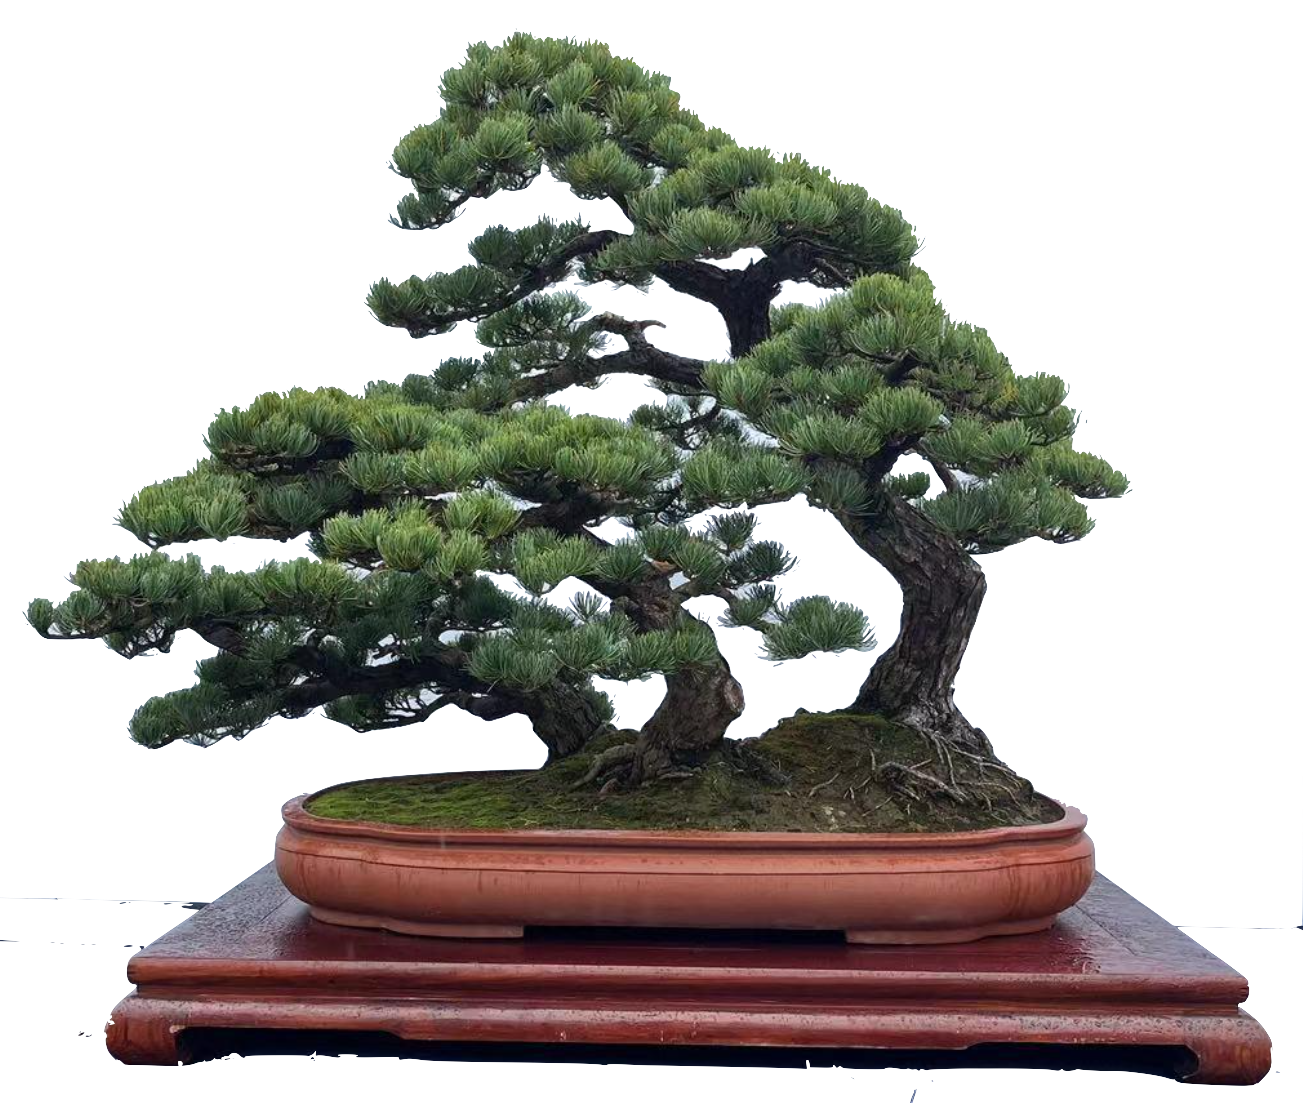
\includegraphics[width=0.95\columnwidth]{res/filler_a.png}
\end{center}

\columnbreak

\topic{December 2025 General TOTM Trees}

\begin{minipage}[b]{.45\textwidth}
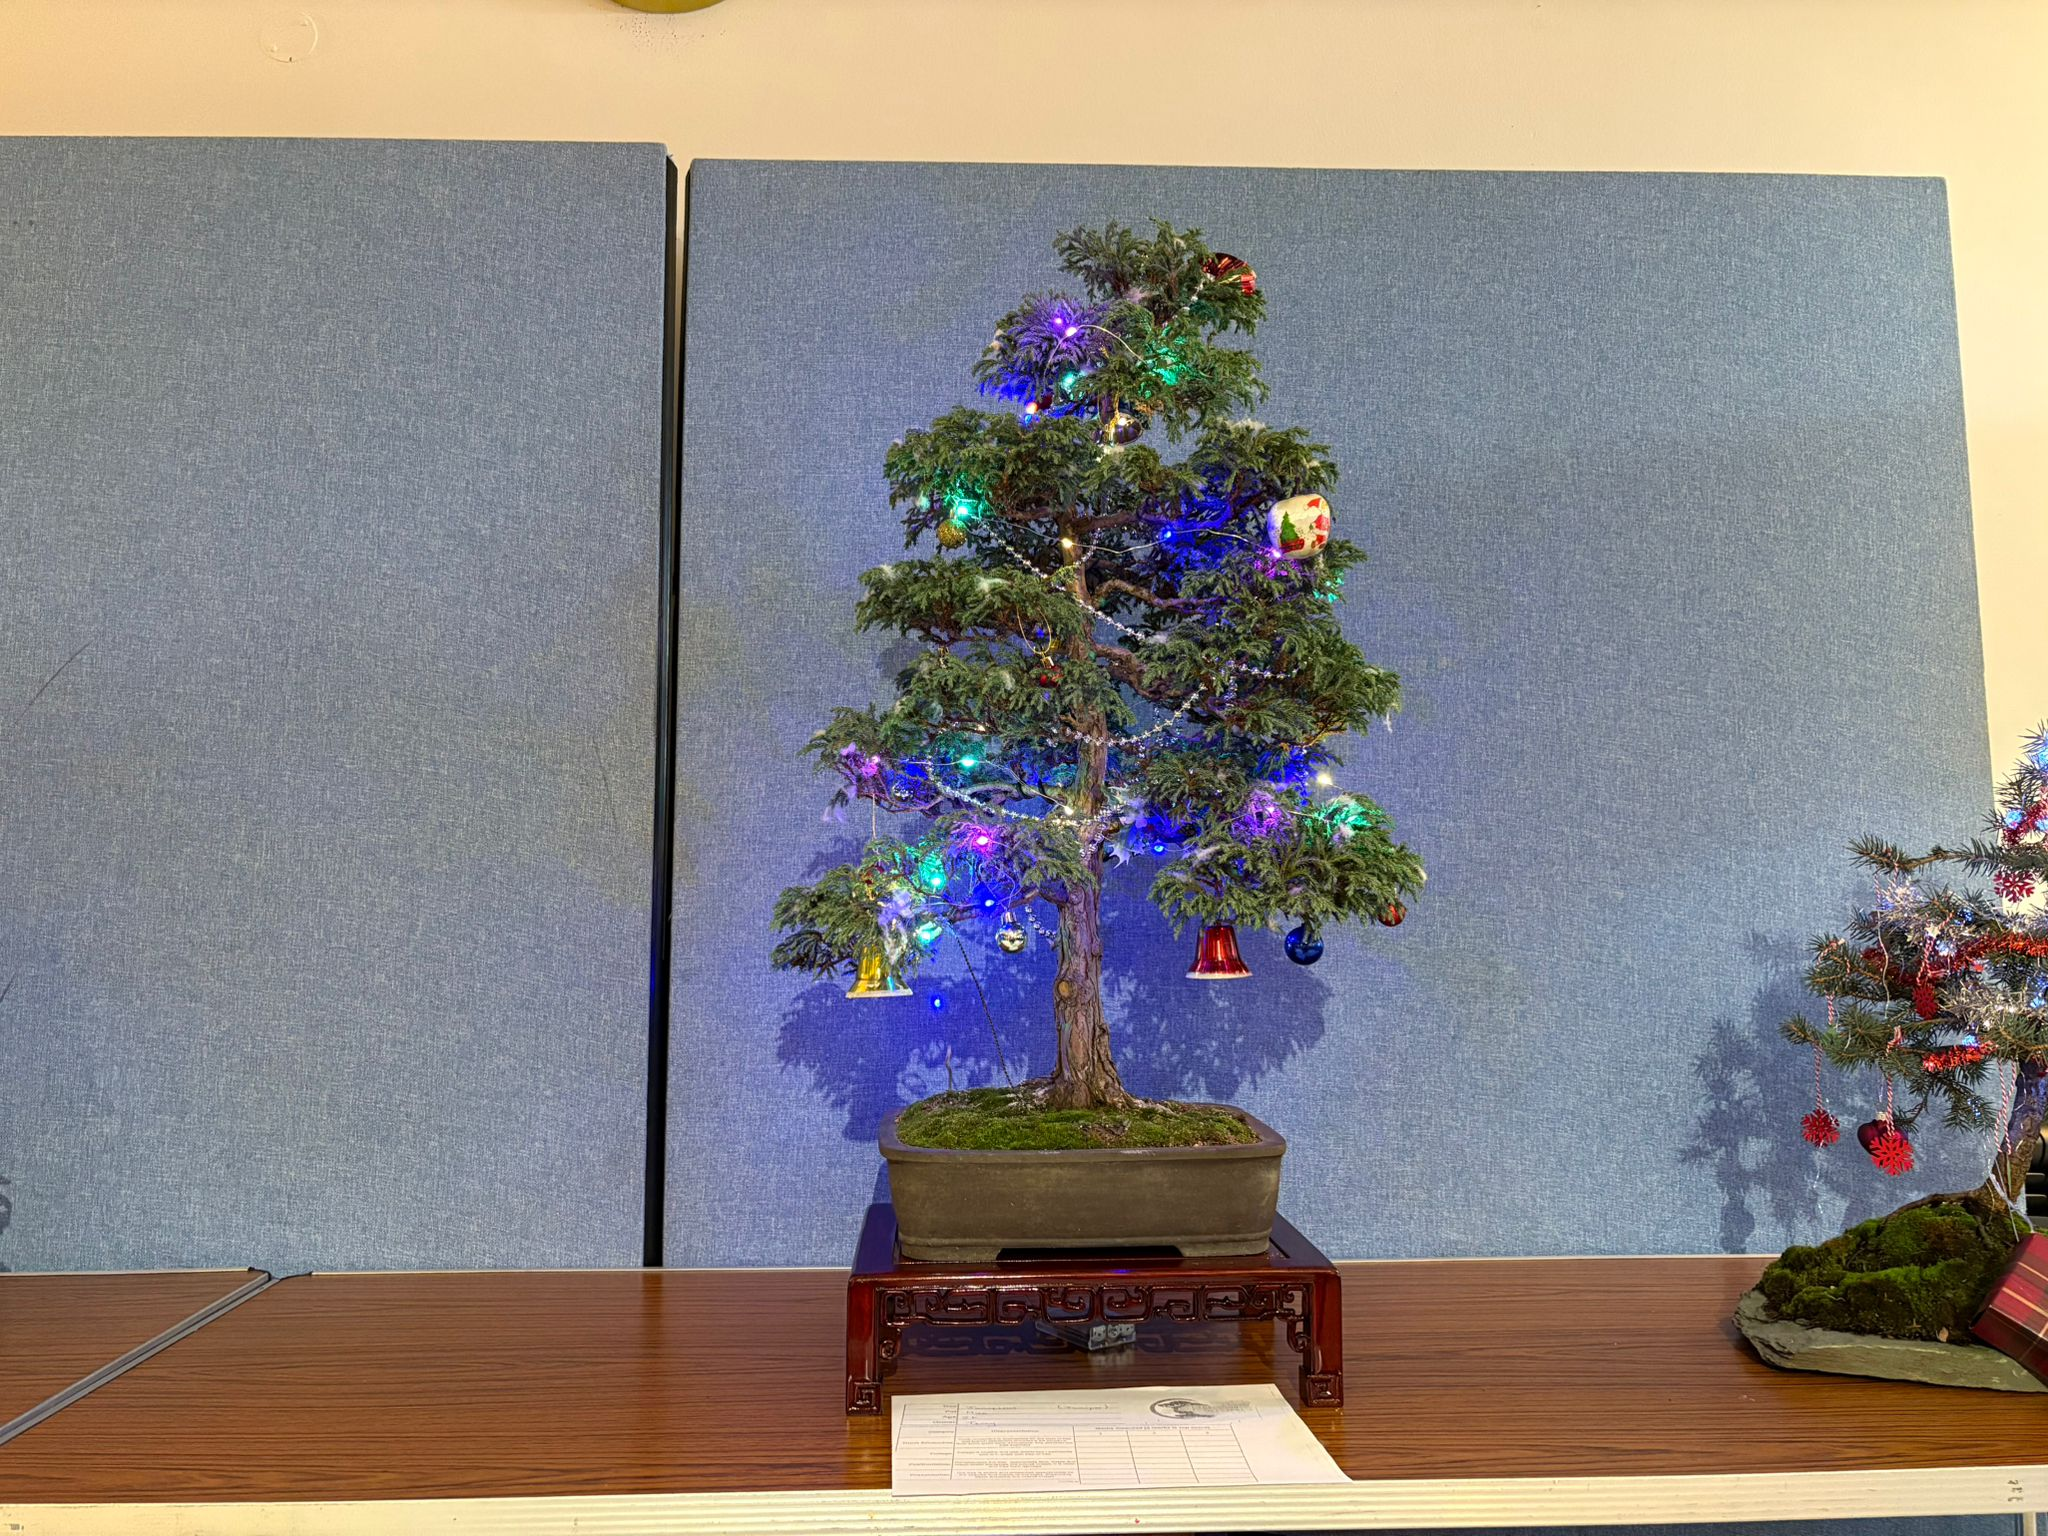
\includegraphics[angle=0,origin=c,width=1.0\textwidth]{2025_12/res/totm_wilson_juniper}
\centerline{\emph{Terry Wilson's Juniper.}}
\end{minipage}
\medskip

\begin{minipage}[b]{.45\textwidth}
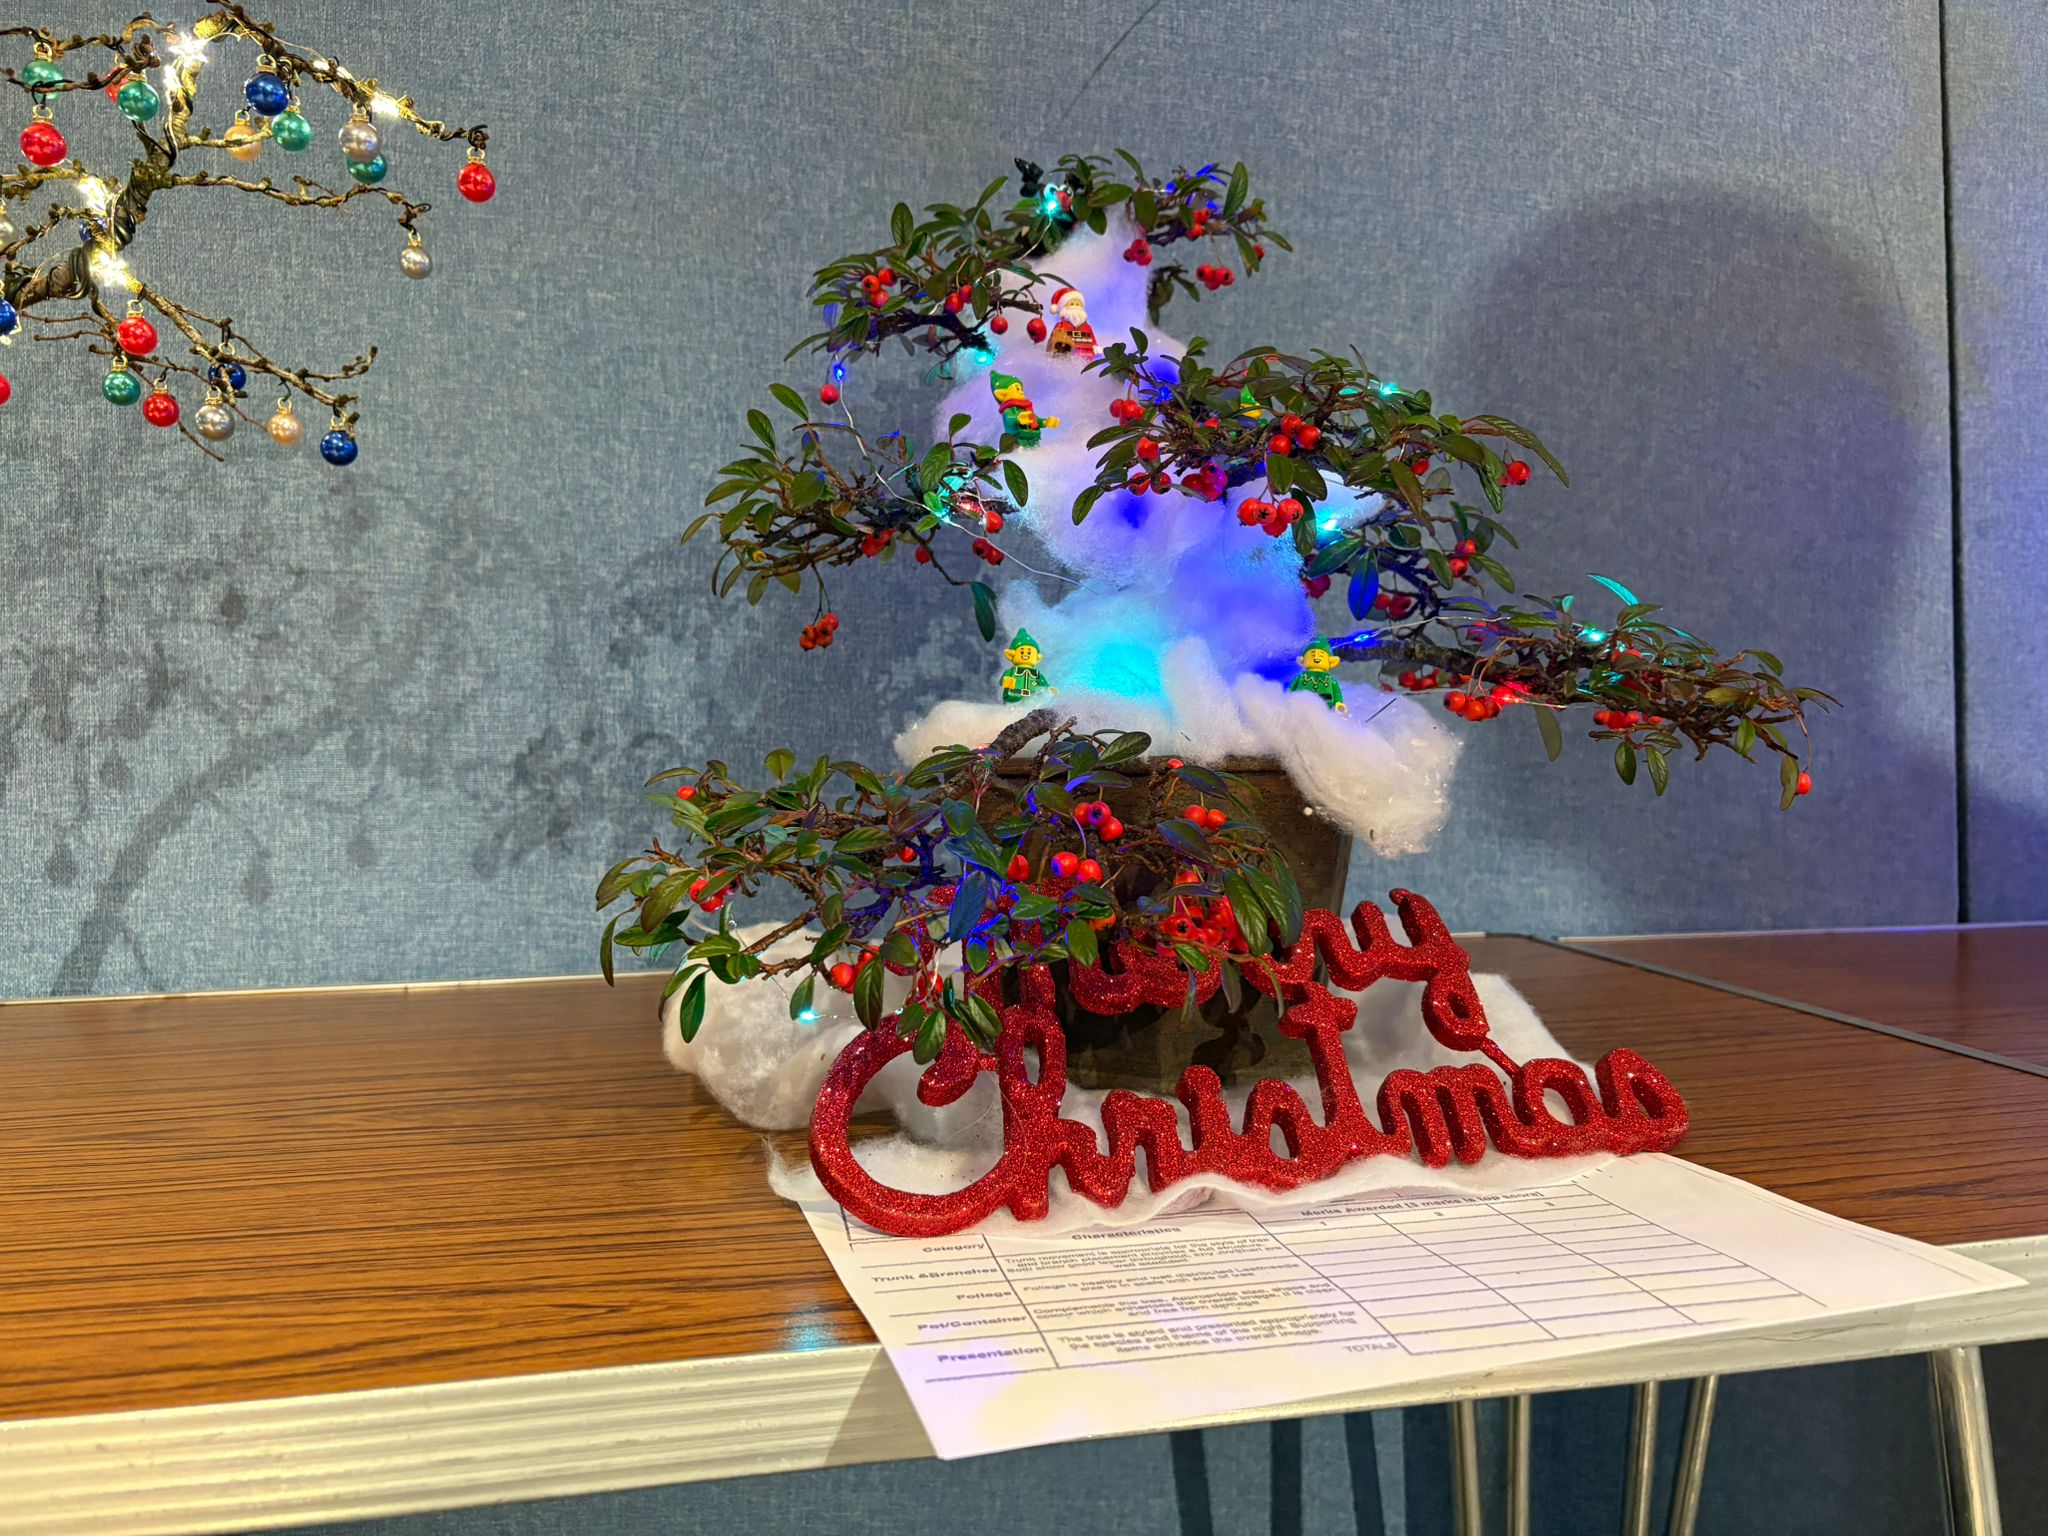
\includegraphics[angle=0,origin=c,width=1.0\textwidth]{2025_12/res/totm_todd_cotoneaster}
\centerline{\emph{Tina Todd's Cotoneaster.}}
\end{minipage}
\medskip

\begin{minipage}[b]{.45\textwidth}
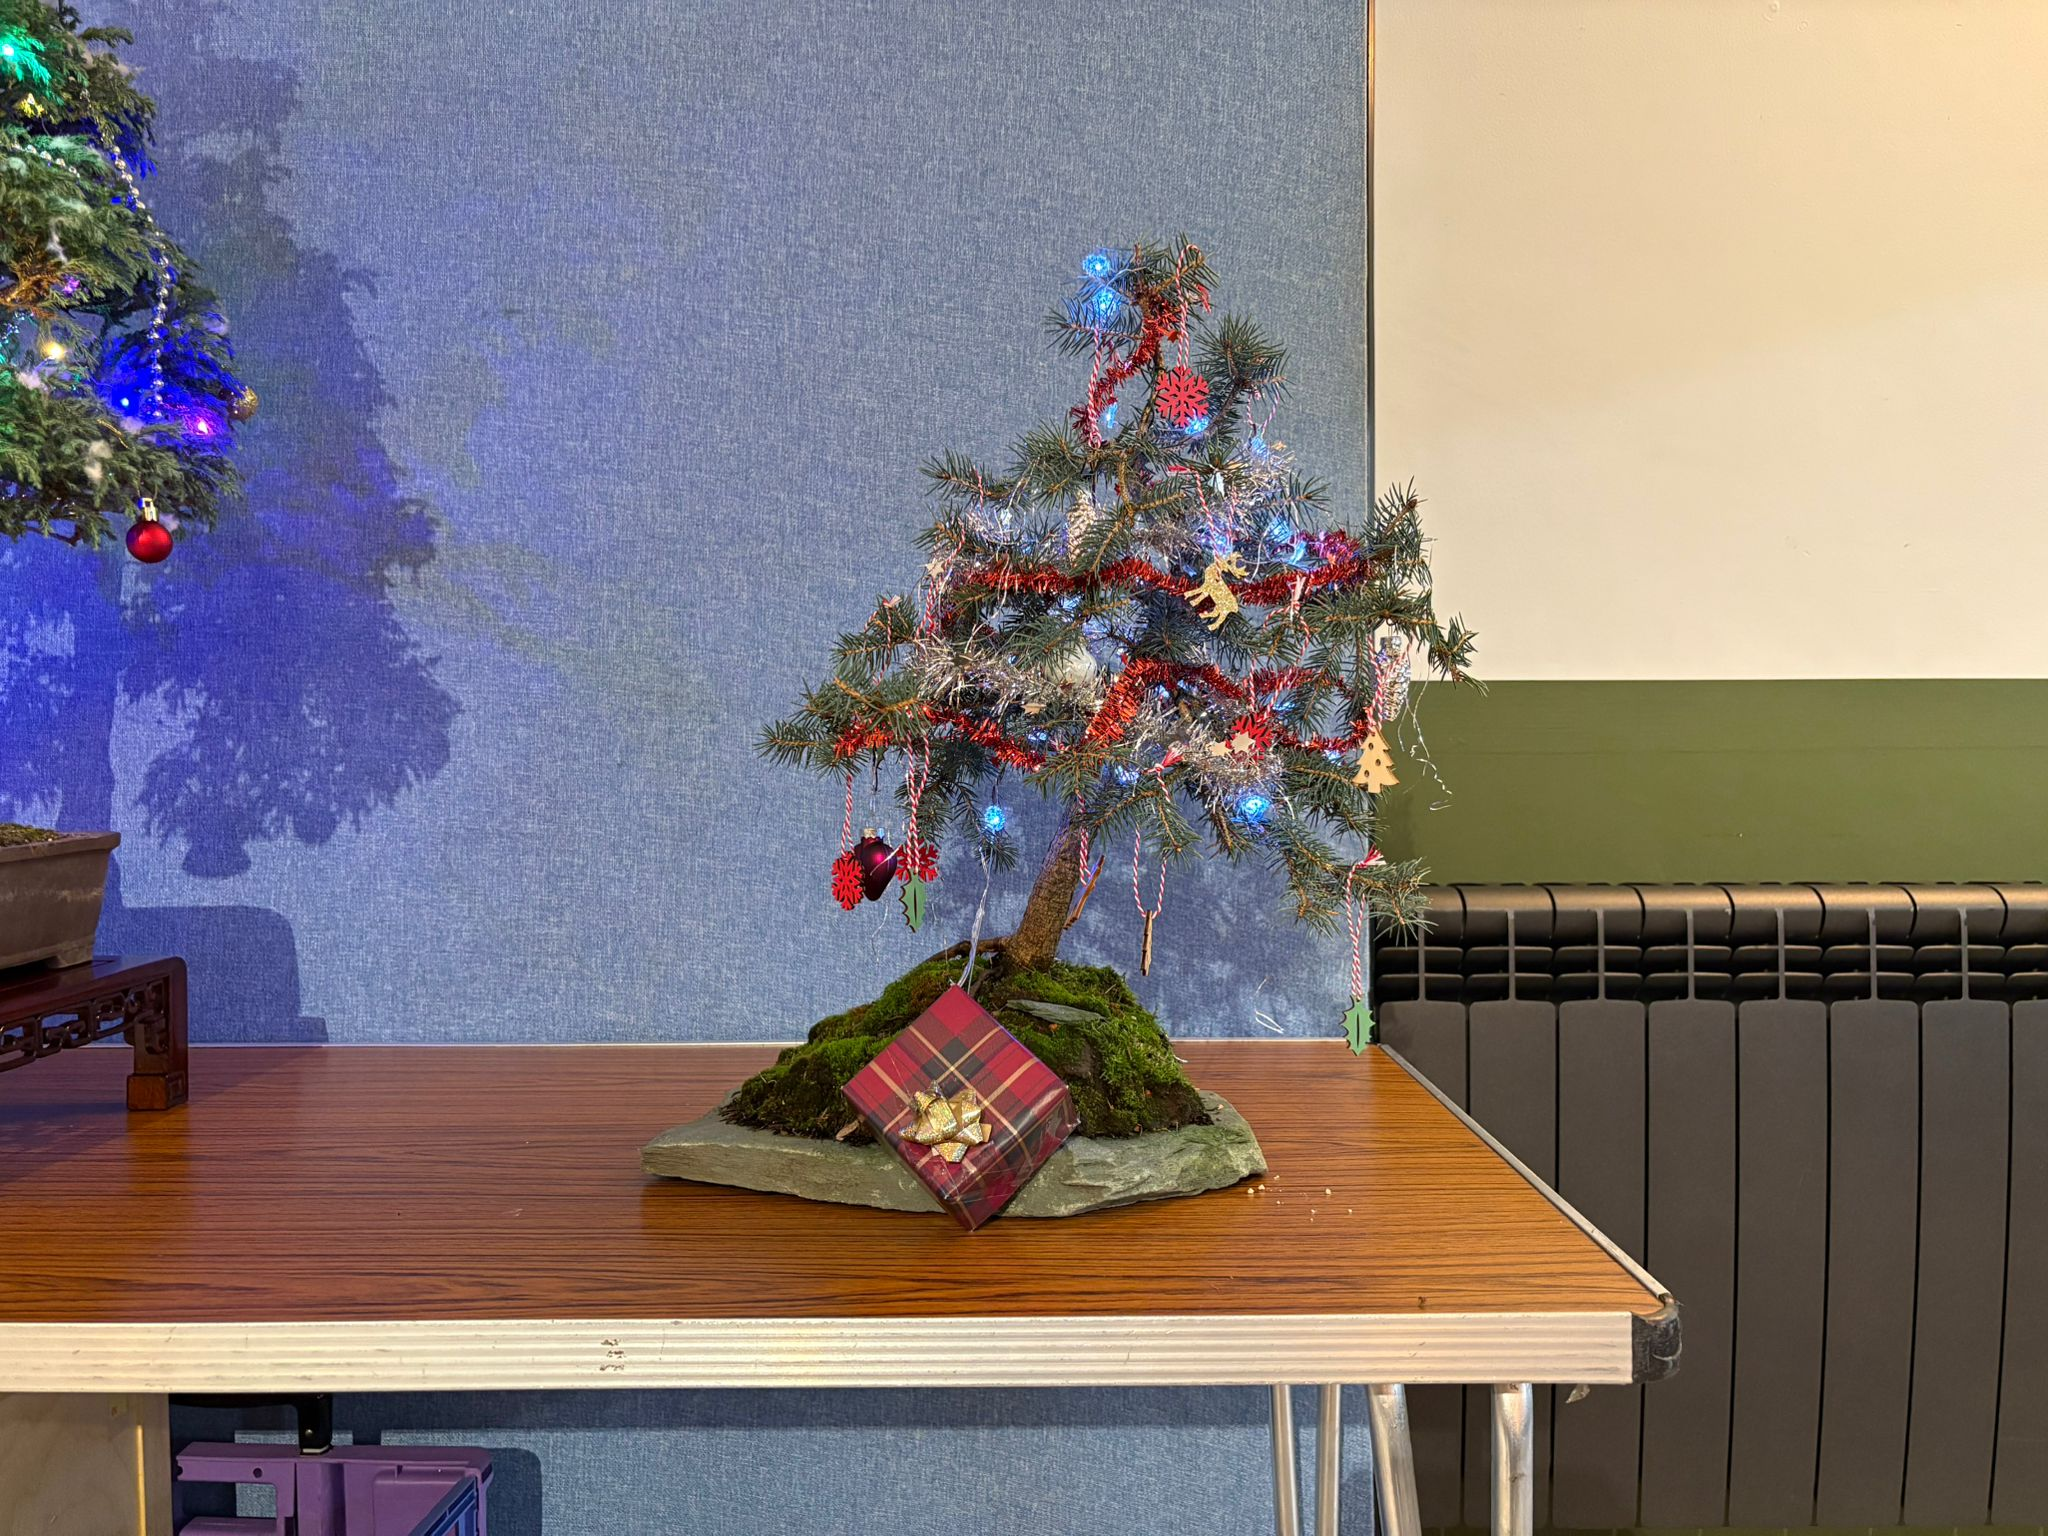
\includegraphics[angle=0,origin=c,width=1.0\textwidth]{2025_12/res/totm_palmer_spruce}
\centerline{\emph{Steve Palmer's White Spruce.}}
\end{minipage}
\medskip

\vfill

\textcolor{white}{space}

\columnbreak

\topic{December 2025 Novice TOTM Trees}

\begin{minipage}[b]{.45\textwidth}
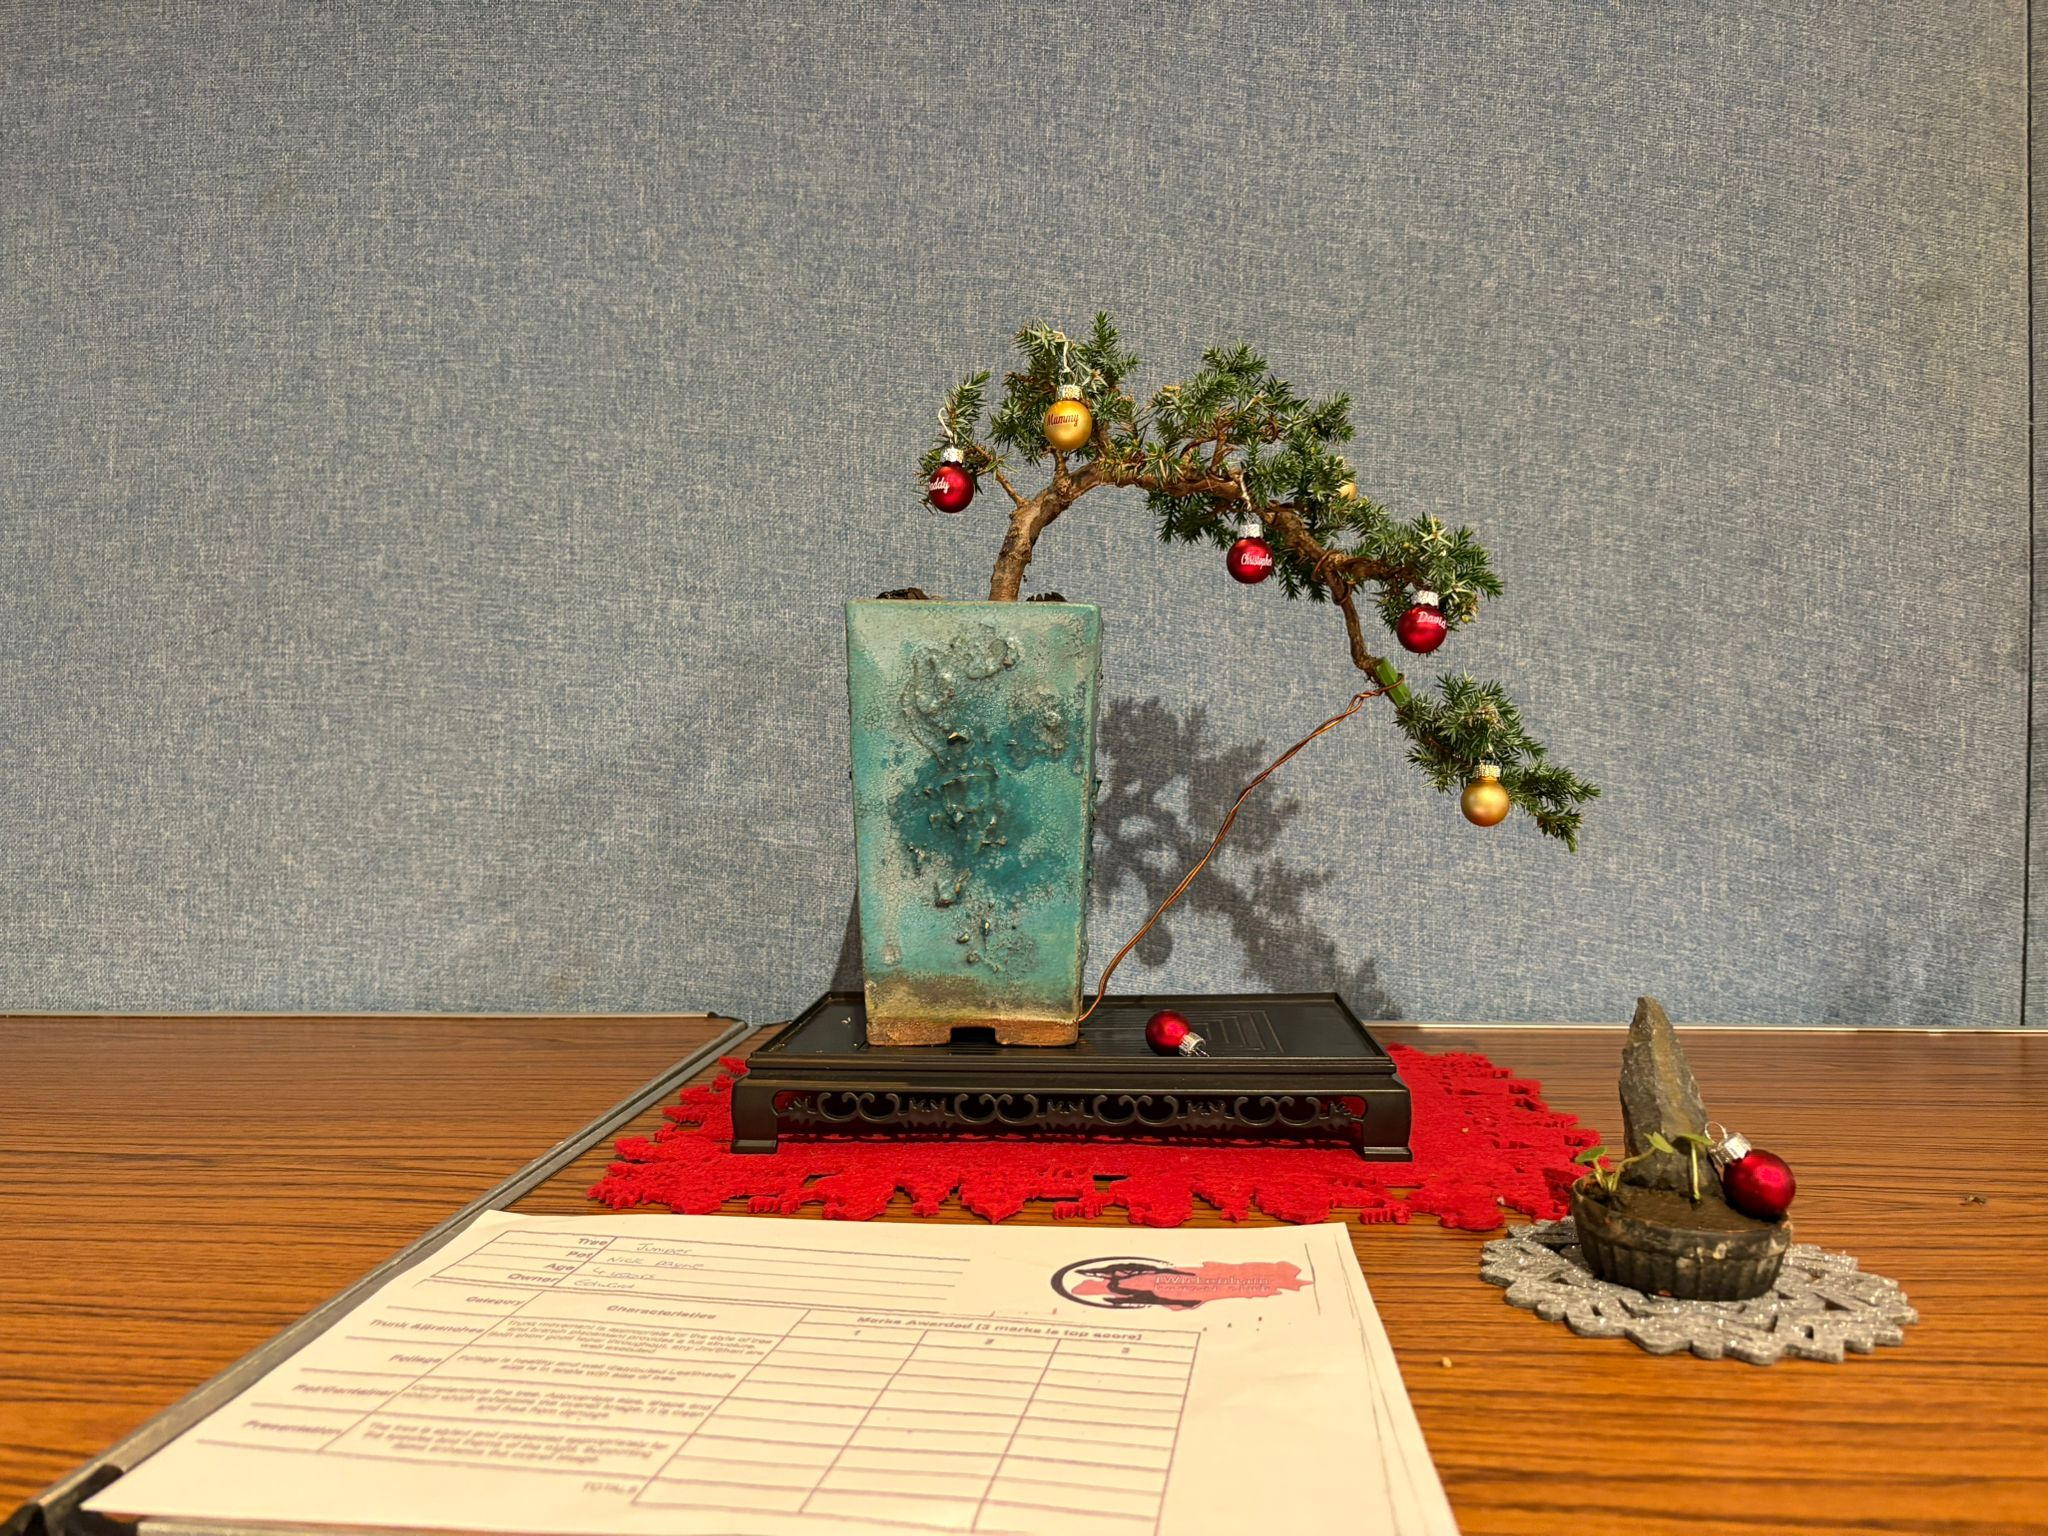
\includegraphics[angle=0,origin=c,width=1.0\textwidth]{2025_12/res/totm_novice_mason_juniper}
\centerline{\emph{Edward Mason's Himalayan Juniper.}}
\end{minipage}
\medskip

\begin{minipage}[b]{.45\textwidth}
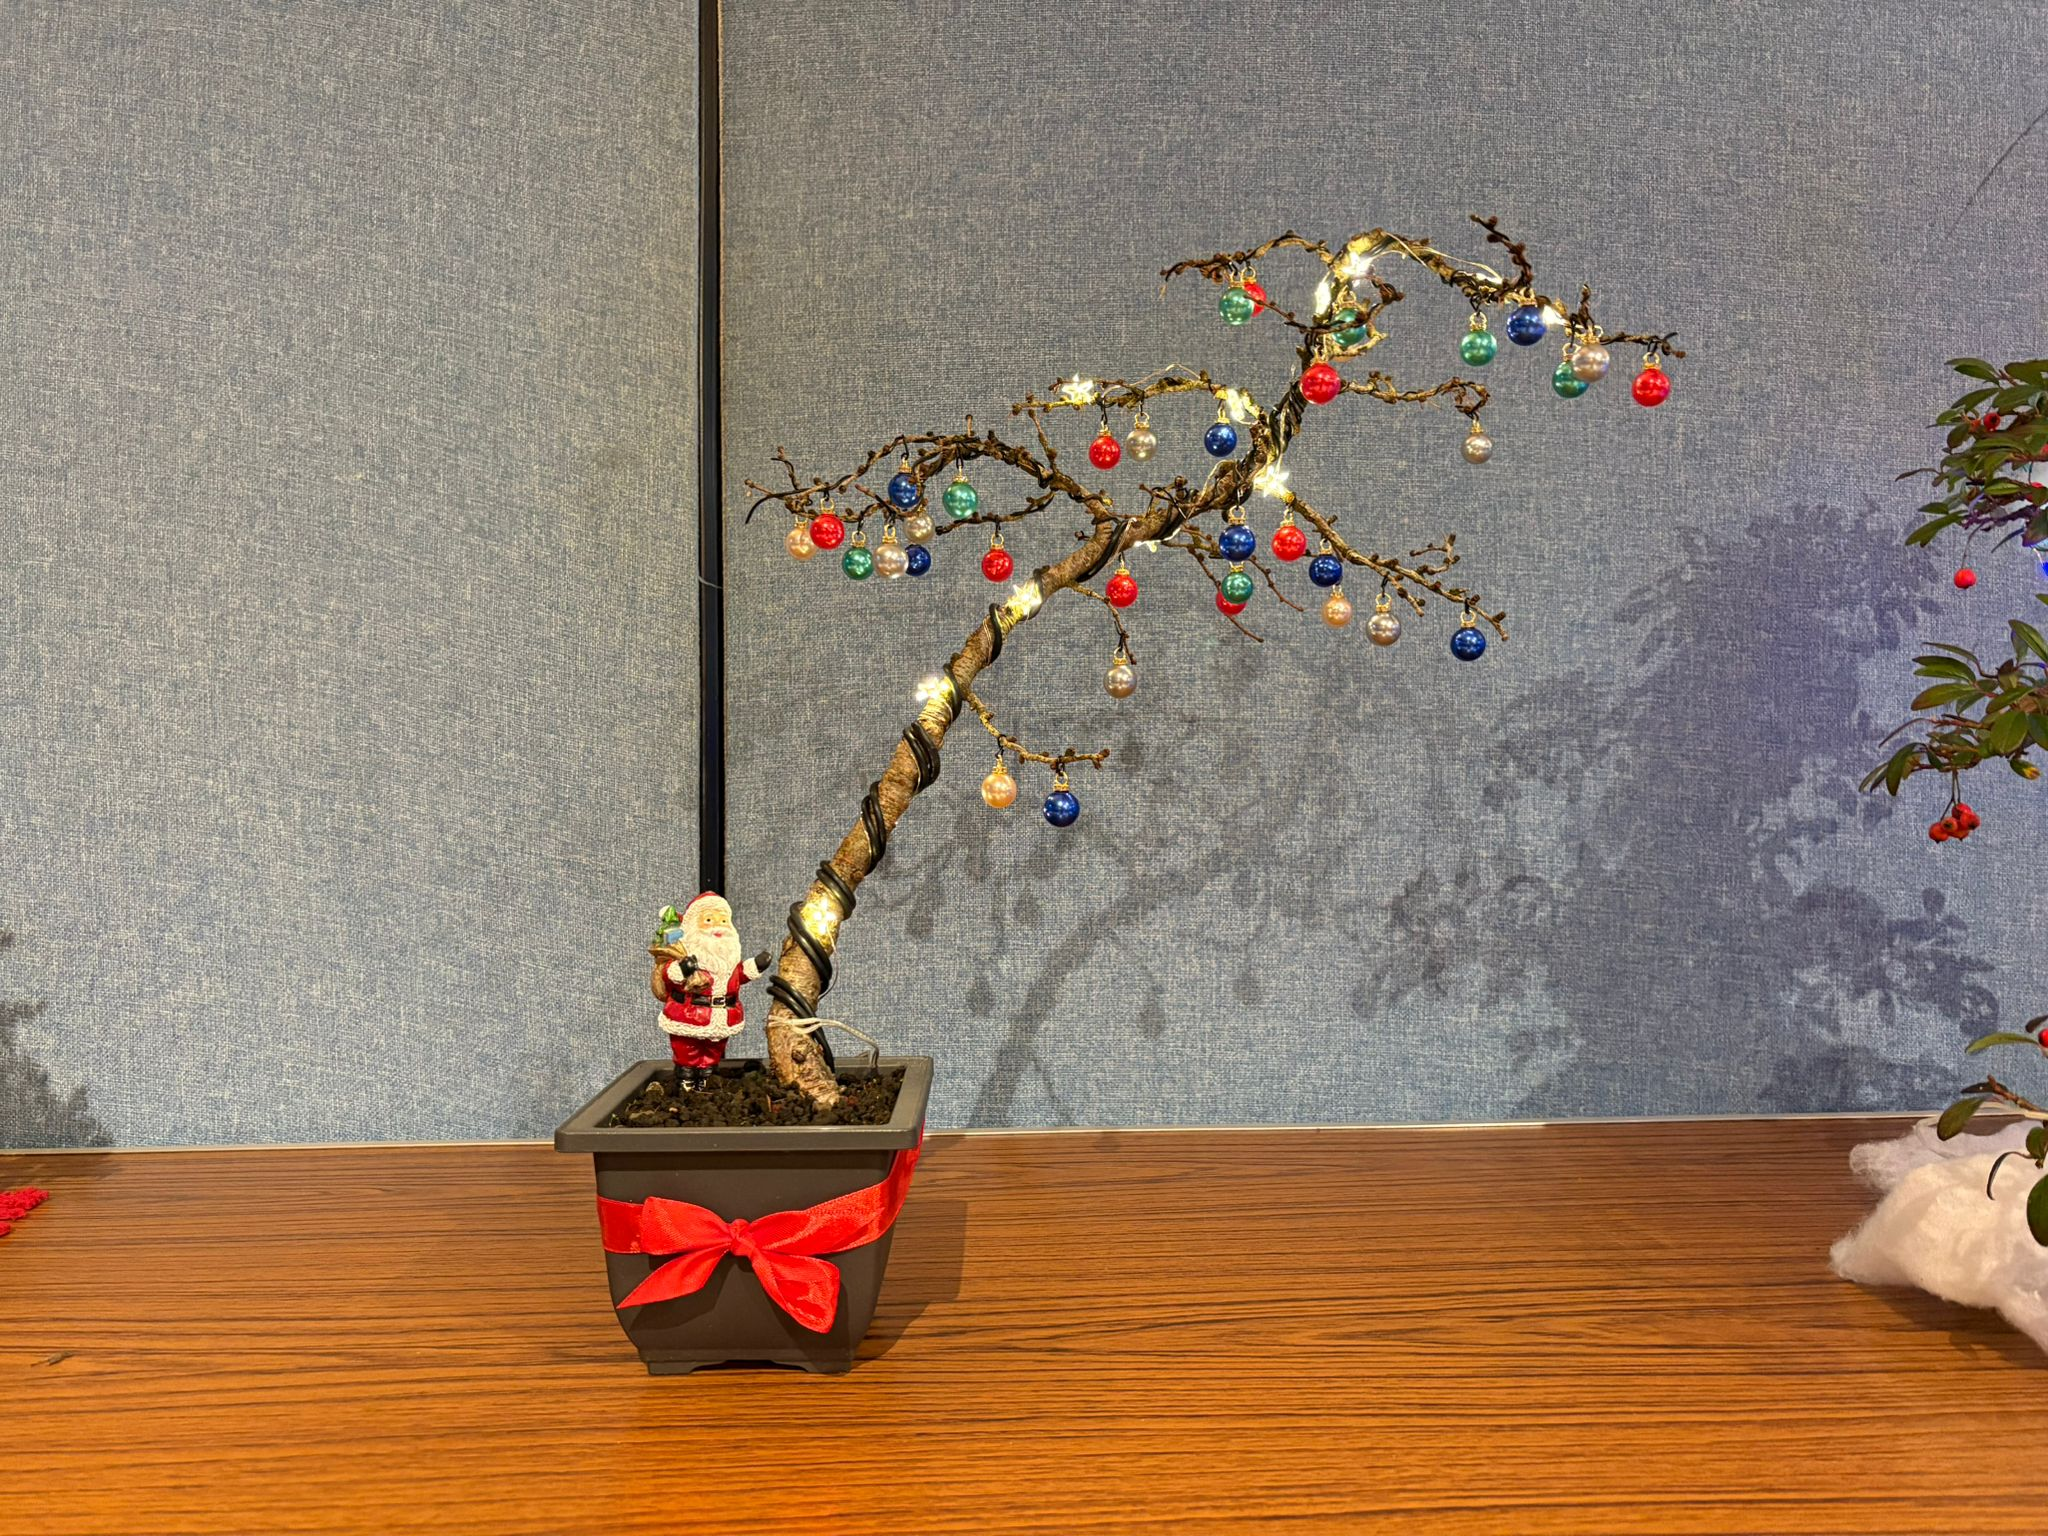
\includegraphics[angle=0,origin=c,width=1.0\textwidth]{2025_12/res/totm_novice_redfern_larch}
\centerline{\emph{Martin Redfern's European Larch.}}
\end{minipage}
\medskip

\clearpage
